\section{Semantic-to-Metric Navigation}
\label{sec:method}

\ours is a navigation agent that instantiates the factorization of \cref{eq:factor}: the VLM is its semantic
sensor, and the agent owns all state and every decision. The belief
$\mathcal{B}_t=(\mathcal{H}_t,M_t)$ consists of a list of target hypotheses $\mathcal{H}_t$ and an occupancy map
$M_t$; \cref{fig:mech} shows one step in full.

\subsection{Per-image questions}
At the start of an episode the VLM $f$ rewrites $\ell$ into a target phrase $s$: the category when the instruction
names or implies one, and the appearance words when it describes only how the object looks. At every step two
queries about the current frame run in parallel. The presence probability is read from the first answer token,
\begin{equation}
\pi_t=\frac{P_f(\textit{yes}\mid I_t,s)}{P_f(\textit{yes}\mid I_t,s)+P_f(\textit{no}\mid I_t,s)},
\label{eq:presence}
\end{equation}
and the second query returns a box $b_t$ for $s$ or none. Neither query contains the action history, the map,
or earlier answers, so every answer can be checked against the image alone.

\noindent\textbf{Lifting.}
A box with centre $c(b_t)=(u,v)$ is lifted with the median depth $\tilde d_t$ over its central half (half its width
and half its height). With focal length $\varphi$ and principal point $(u_0,v_0)$ of the pinhole camera, tilt
$\phi_t$, and the forward and right unit vectors $e_f(\theta_t),e_r(\theta_t)$ of the heading,
\begin{equation}
q_t=x_t+\tilde d_t\Big[\big(\cos\phi_t-\tfrac{v-v_0}{\varphi}\sin\phi_t\big)\,e_f(\theta_t)
+\tfrac{u-u_0}{\varphi}\,e_r(\theta_t)\Big],
\label{eq:lift}
\end{equation}
which we write $q_t=\Pi_{p_t}^{-1}(c(b_t),\tilde d_t)$; lifts with $\tilde d_t>6$\,m are discarded. The same
back-projection, with the known camera height, labels each depth pixel as floor (height below 0.10\,m) or obstacle
(0.10--1.9\,m) in a 5\,cm occupancy grid $M_t$.

\noindent\textbf{Observation weight.}
A lifted box enters the memory with weight
\begin{equation}
a_t=\begin{cases}\pi_t & \text{if the target is named and } \pi_t\ge\tfrac12,\\
\pi^z_t & \text{otherwise, if } \pi^z_t\ge\tfrac12,\\
0.2\,\pi^z_t & \text{otherwise,}\end{cases}
\label{eq:weight}
\end{equation}
where $\pi^z_t$ is the presence probability of a \emph{crop check}, a square crop of 2.5 times the box's longer
side resized to 448\,px. The crop is queried only when presence and box disagree or when the goal is
appearance-only, so the extra cost is paid where the evidence is weak.

\subsection{Metric hypothesis memory}
Each hypothesis $k$ stores a floor position $\mu_k$, evidence $w_k$, and the poses $V_k$ from which it was seen. An
observation $(q_t,a_t)$ is associated with the first hypothesis within \mbox{$r=0.5$\,m}. If there is one, then
\begin{equation}
\mu_k\leftarrow\frac{n_k\mu_k+q_t}{n_k+1},\qquad w_k\leftarrow w_k+\gamma_t\,a_t ,
\label{eq:fuse}
\end{equation}
with $n_k$ the number of fused observations and $\gamma_t=0.25$ if some $v\in V_k$ has the heading of $p_t$ and a
position within 0.2\,m of it, else $\gamma_t=1$; otherwise a new hypothesis $(\mu,w)=(q_t,a_t)$ is created. Through $\gamma_t$, evidence grows with the number
of distinct viewpoints rather than with the number of frames.

\noindent\textbf{Commitment and exhaustion.}
The agent commits to a hypothesis once $w_k\ge\tau_c=0.8$ and keeps it while $w_k\ge\tau_k=0.4$; the hysteresis
prevents one missed detection from abandoning a well-supported target. When the agent stands within 0.9\,m of a
committed hypothesis and the episode continues, which on EB-Navigation means that it is not the target, the
hypothesis is marked exhausted. It stays in memory, so later detections of the same look-alike merge into it
instead of creating a new target.

\subsection{Search and control}
\noindent\textbf{Selection and look-around.}
The agent heads for the committed hypothesis with the largest evidence. With nothing committed, it approaches the
strongest hypothesis with $w_k\ge0.35$ when that hypothesis is detected in the current frame. Otherwise it turns
through the three remaining headings, so that a target behind it enters the view, then approaches the strongest
hypothesis with $w_k\ge0.35$, and otherwise moves to the observed free cell 0.75--3\,m away that is farthest from
all visited positions and looks around again. A weak target already in view is thus inspected before the agent
turns away from it.

\noindent\textbf{Planning.}
Actions come from A* over (position, heading) on $M_t$, whose edges are the benchmark's translations and turns.
An edge costs 1 plus 0.15 for each of four sampled points on it that is unobserved; edges through inflated
obstacles are removed, and a move that the simulator has rejected becomes a forbidden edge.

\begin{table*}[t]
\centering\small
\setlength{\tabcolsep}{5pt}\renewcommand{\arraystretch}{0.92}
\caption{Success rate (\%) on EB-Navigation test. Top: reported results. Bottom: our runs on one 8\,GB GPU, with \ours at 4-bit. $\pm$: std.\ over test runs. Bold: best of our runs per model.}
\label{tab:main}
\sbox0{\begin{tabular}{@{}llrrrrrr@{\,}lc@{}}
\toprule
Method & Model & Base & Common & Complex & Visual & Long & Avg. & & 95\% CI\\
\midrule
\multicolumn{10}{@{}l}{\textit{Prompted MLLMs (EmbodiedBench)}}\\
EB prompt~\cite{yang2025embodiedbench} & GPT-4o & 55.0 & 60.0 & 58.3 & 60.0 & 55.0 & 57.7 & & --\\
EB prompt~\cite{yang2025embodiedbench} & InternVL3-78B & 66.7 & 63.3 & 61.7 & 45.0 & 31.7 & 53.7 & & --\\
EB prompt~\cite{yang2025embodiedbench} & Gemini-2.0-flash & 63.3 & 65.0 & 50.0 & 51.7 & 13.3 & 48.7 & & --\\
EB prompt~\cite{yang2025embodiedbench} & Claude-3.7-Sonnet & 50.0 & 61.7 & 50.0 & 36.7 & 26.7 & 45.0 & & --\\
EB prompt~\cite{yang2025embodiedbench} & Qwen2.5-VL-72B & 46.7 & 46.7 & 46.7 & 26.7 & 33.3 & 40.0 & & --\\
EB prompt~\cite{yang2025embodiedbench} & InternVL3-8B & 38.3 & 30.0 & 40.0 & 33.3 & 5.0 & 29.3 & & --\\
EB prompt~\cite{yang2025embodiedbench} & Qwen2.5-VL-7B & 20.0 & 26.7 & 38.3 & 16.7 & 0.0 & 20.3 & & --\\
\multicolumn{10}{@{}l}{\textit{Training-free agents}}\\
MOSAIC (module graph)~\cite{wang2026mosaic} & Qwen3-VL-8B & 60.0 & 46.7 & 45.6 & 51.1 & 46.7 & 50.0 & & --\\
ESCA (scene graph)~\cite{huang2025esca} & GPT-4o & 66.7 & 62.0 & 63.3 & 55.0 & 26.7 & 54.7 & & --\\
EmbodiSkill (skills)~\cite{ju2026embodiskill} & Qwen3-VL-32B & 65.0 & 68.0 & 73.0 & 67.0 & 33.0 & 61.3 & & --\\
RoboFoundry (self-evolving)$^\|$~\cite{liang2026robofoundry} & Qwen3.8-27B & 76.7 & 85.0 & 73.3 & 63.3 & 43.3 & 68.3 & & --\\
BrainMem (memory)~\cite{ma2026brainmem} & GPT-4o & 73.3 & 71.7 & 80.0 & 66.6 & 63.3 & 71.0 & & --\\
EMHO (harness)$^\P$~\cite{lee2026emho} & Qwen3.8-27B & 86.7 & 76.7 & 73.3 & 76.7 & 63.3 & 75.3 & & --\\
RoboFoundry (self-evolving)$^\|$~\cite{liang2026robofoundry} & GPT-6 Astra & 90.0 & 85.0 & 86.7 & 73.3 & 66.7 & 80.3 & & --\\
Tool library~\cite{zhou2026enabling} & Qwen3-VL-8B & 85.0 & 85.0 & 77.0 & 75.0 & 77.0 & 80.0 & & --\\
Tool library~\cite{zhou2026enabling} & GPT-4o & 80.0 & 85.0 & 85.0 & 80.0 & 83.0 & 83.0 & & --\\
\multicolumn{10}{@{}l}{\textit{Fine-tuned}}\\
SVA (Q-model)$^\P$~\cite{xie2026sva} & Qwen3.5-4B & 54.2 & 41.7 & 45.8 & 41.7 & 50.0 & 46.7 & & --\\
MuSix (world models)$^\P$~\cite{jang2026musix} & Qwen3-VL-4B & 63.2 & 63.2 & 57.6 & 62.4 & 43.2 & 57.9 & & --\\
\midrule
\multicolumn{10}{@{}l}{\textit{Ours (one 8\,GB GPU)}}\\
EB prompt & Qwen3-VL-4B & 66.7 & 65.0 & 65.0 & 53.3 & 25.0 & 55.0 &  & [49.3, 60.7]\\
Modular, single view$^\S$ & Qwen3-VL-4B & 68.3 & 66.7 & 68.3 & 50.0 & 70.0 & 64.7 &  & [59.3, 70.0]\\
\ours{}$^\S$ & Qwen3-VL-4B & \textbf{87.8} & \textbf{83.9} & \textbf{85.0} & \textbf{59.4} & \textbf{80.0} & \textbf{79.2} & {\scriptsize$\pm$0.7} & [74.7, 83.6]\\
\ours, RGB only$^\dagger$ & Qwen3-VL-4B & 83.3 & 80.0 & 80.0 & 59.2 & 77.5 & 76.0 & {\scriptsize$\pm$0.9} & [71.2, 80.7]\\
\midrule
EB prompt & Qwen2.5-VL-3B & 21.7 & 21.7 & 28.3 & 20.0 & 10.0 & 20.3 &  & [16.0, 25.0]\\
\ours{}$^\S$ & Qwen2.5-VL-3B & \textbf{76.7} & \textbf{68.3} & \textbf{73.3} & \textbf{51.7} & \textbf{75.0} & \textbf{69.0} &  & [63.7, 74.0]\\
\midrule
EB prompt & Qwen3-VL-2B & 41.7 & 36.7 & 41.7 & 33.3 & 15.0 & 33.7 &  & [28.3, 39.0]\\
\ours{}$^\S$ & Qwen3-VL-2B & 86.7 & \textbf{76.7} & \textbf{81.7} & \textbf{60.0} & \textbf{80.0} & \textbf{77.0} &  & [72.3, 81.7]\\
\ours, RGB only$^\dagger$ & Qwen3-VL-2B & \textbf{88.3} & \textbf{76.7} & \textbf{81.7} & 55.0 & 76.7 & 75.7 &  & [70.7, 80.3]\\
\midrule
Oracle target$^\ddagger$ & -- & 93.3 & 93.3 & 93.3 & 93.3 & 83.3 & 91.3 &  & [88.0, 94.3]\\
\bottomrule
\end{tabular}}\usebox0

\vspace{0.2em}\parbox{\wd0}{\footnotesize $^\S$Depth sensor and simulator pose. $^\dagger$RGB only: monocular depth and pose from the executed actions (\cref{sec:sensing}); the comparisons with reported results use this row. $^\ddagger$Geometric planner given the true target position: an upper bound. $^\P$Reported on part of each subset: the best held-out score over search iterations on half of it (EMHO), or episodes 36--60 (MuSix) and 37--60 (SVA), on which \ours (RGB only) reaches \nRGBMuSix\% and \nRGBSVA\%. $^\|$Edits its prompts and code while it runs on the test episodes.}
\end{table*}


\begin{figure*}[t]
\centering
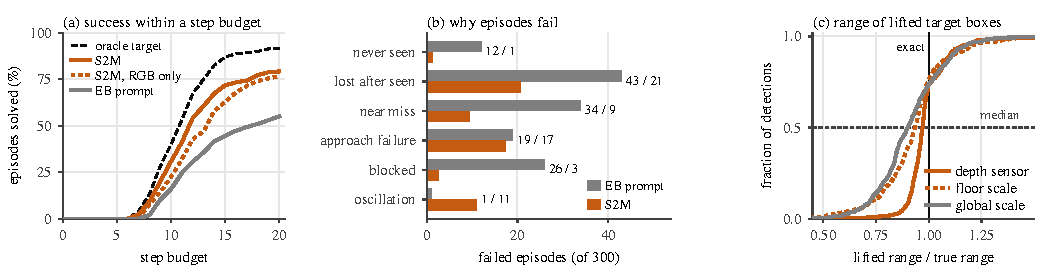
\includegraphics[width=\textwidth]{fig/analysis.pdf}
\caption{EB-Navigation test, Qwen3-VL-4B. \textbf{(a)} Episodes solved within a step budget, averaged over runs.
\textbf{(b)} Failed episodes by outcome (first matching rule, \cref{sec:diagnosis}; mean over the runs of \ours).
\textbf{(c)} Cumulative distribution of lifted over true range for detections within 1\,m of the target (dashed:
median), with the depth sensor and with monocular depth under a per-frame floor scale (\cref{eq:floorscale}) or a
global scale.}
\label{fig:analysis}
\end{figure*}

\subsection{RGB-only and explicit-stop variants}
\label{sec:rgbonly}
Monocular metric depth networks err mostly by a frame-dependent scale. Let $\hat D_t$ be the raw prediction and
$\kappa(v)=\sin\phi_t+\frac{v-v_0}{\varphi}\cos\phi_t$ the downward component of the ray through row $v$ per unit of
planar depth. A pixel on the floor satisfies $\sigma\hat D_t(u,v)\,\kappa(v)=h$ for the camera height $h$, and an
object standing on the floor gives a larger $\sigma$. Over the pixels $\mathcal{F}_t$ whose rays point at least
15$^\circ$ below the horizontal, \ours takes the mode
\begin{equation}
\sigma_t=\operatorname*{mode}_{(u,v)\in\mathcal{F}_t}\ \frac{h}{\hat D_t(u,v)\,\kappa(v)},\qquad D_t=\sigma_t\,\hat D_t ,
\label{eq:floorscale}
\end{equation}
with the mode taken over values in $[\bar\sigma/1.33,\,1.33\,\bar\sigma]$, where $\bar\sigma$ is one global scale
fitted on development frames; it keeps $\bar\sigma$ when fewer than 10\% of the pixels in $\mathcal{F}_t$ fall in
this window. This is the ground-plane constraint of monocular visual
odometry~\cite{song2014robust} applied per frame. Pose comes from dead reckoning over the executed actions,
\begin{equation}
\hat x_{t+1}=\hat x_t+0.25\,o_t\big(\alpha_f e_f(\hat\theta_t)+\alpha_r e_r(\hat\theta_t)\big),
\label{eq:deadreckon}
\end{equation}
with $(\alpha_f,\alpha_r)\in\{(\pm1,0),(0,\pm1)\}$ the translation of $u_t$, and heading and tilt advanced by the
turn or tilt of $u_t$ when $o_t=1$.

\noindent\textbf{Explicit stopping.}
EB-Navigation ends an episode on success; RoboTHOR requires a Stop action. There the agent stops only when it is
within 0.9\,m of a committed hypothesis, has turned within 20$^\circ$ of it and tilted it into view, and a fresh
presence query exceeds 0.5; otherwise the hypothesis is exhausted. Because RoboTHOR episodes last up to 500 steps
and a stop is final, the RoboTHOR agent, frozen before the EB-Navigation agent was simplified, also lowers the
evidence of a hypothesis that a frame within 3\,m shows but does not detect, searches magnified tiles when a view
yields nothing, and explores toward the nearest frontier (supplement).
